% Ötödik előadás

\chapter{Processzor szintű fizikai architektúra}

\section{Részei}
\begin{itemize}
    \item műveletvégző
    \item vezérlő
    \item I/O rendszer
    \item megszakításrendszer
\end{itemize}
A legfontosabbak a műveletvégző és a vezérlő részek, mivel ezek végzik a CPU két fő funkcióját (utasítás lehívás és végrehajtás).

\section{Szinkron és aszinkron CPU-k}
Kétféle CPU-t különböztetünk meg:
\begin{itemize}
    \item aszinkron: nincs órajel, hanem az utasítás vége jelzés a következő utasítás megkezdésére. Előnye, hogy nincs holtidő, hátránya hogy az utasítás végének érzékeléséhez speciális áramkörök kellenek, ami viszonylag drága és az érzékelés is időt vesz igénybe.
    \item szinkron: a végrehajtást órajel vezérli
\end{itemize}

\section{Műveletvégző egység}
A műveletvégző egység tartalmazza a:
\begin{itemize}
    \item regisztereket
    \item adatutakat
    \item kapcsolópontokat
    \item szűkebb értelemben vett ALU-t
\end{itemize}

\subsection{Regiszterek}
A műveletvégző egység tartalmaz látható és transzparens regisztereket.
Láthatóból megkülönböztetünk univerzális és dedikált (pl. stack) regisztereket.
A transzparens (rejtett) regiszterek általában az adatfeldolgozáshoz szükséges puffer regiszterek.
A rejtett regiszterekre nem lehet hivatkozni, de számításba kell venni őket alacsony szintű programozásnál.

\subsection{Adatutak}
Ez nem adatbusz!
Az adatbuszon értelmezett a címzés, adatutak esetén viszont nem beszélhetünk címzésről.
Az adatutak a műveletvégző egység részeit kapcsolja össze, gyakorlatilag egy vezetékrendszer.

\subsection{Kapcsolópontok}
A regiszterkhez kapcsolópontokon keresztül csatlakoznak a vezetékek.
A kapcsolók tranzisztorok, a regiszterek részei.
A kimeneti kapcsoló három állású: zárt, nulla és egy.
A bemeneti kapcsoló kétállású: nyitott és zárt.
Az adatutakon egyszerre csak egy adat lehet, ezért a kapcsolópontok felelnek azért, hogy csak a megfelelő regiszter legyen nyitva.
A vezérlő nyitja és zárja a kapcsolókat.

\subsection{Csatolási módok}
Az adatutakat csoportosíthatjuk csatolási mód szerint:
\begin{itemize}
    \item egyutas
    \item kétutas
    \item háromutas
\end{itemize}

\subsubsection{Egyutas csatolás}
Előnye, hogy egyszerű és olcsó, hátránya, hogy lassú.
\begin{figure}[H]
    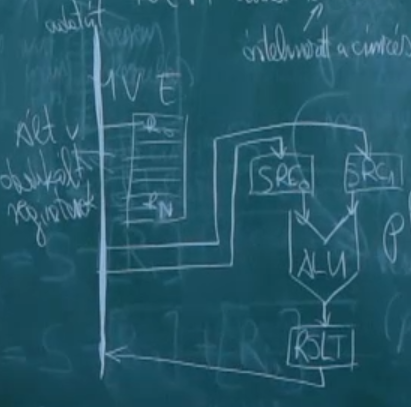
\includegraphics[width=0.8\textwidth]{adatut}
    \centering
    \caption{Egyutas adatút}
    \label{fig:adatut}
\end{figure}
Példa egyutas adatút működésére ADD r0,r1 művelet esetén:
\begin{enumerate}
    \item Az R0 tartalmát be kell tölteni az egyik forrásregiszterbe, ezért a vezérlő megnyitja R0 és SRC0 kapcsolóit, hogy az adatúton keresztül a jel eljuthasson.
    \item Ezután jön R1, itt R1 és SRC1 kapcsolóit nyitja a vezérlő.
    \item Szinkronizáltan, órajelre megnyílnak SRC0 és SRC1 kimenő kapcsolói, a forrás operandusok eljutnak az ALU-ba, ahol megtörténik az összeadás.
    \item Az ALU-ból bekerül az adat az eredményregiszterbe.
    \item Végül az eredmény visszajut R0-ba.
\end{enumerate}

\subsubsection{Kétutas csatolás}
A kétutas csatolás használatával egyszerre tölthető be a két operandus, így a betöltési idő a felére csökken.
\begin{figure}[H]
    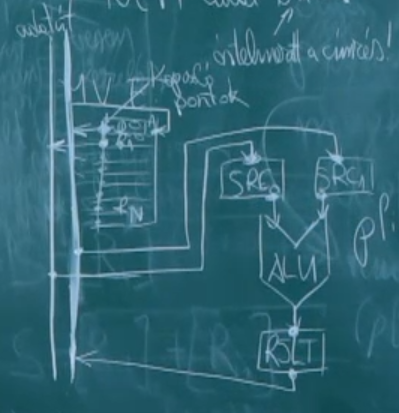
\includegraphics[width=0.8\textwidth]{ketut}
    \centering
    \caption{Kétutas adatút}
    \label{fig:ketut}
\end{figure}

\subsubsection{Háromutas csatolás}
Itt a harmadik adatút a kimenetre van rákötve.
Ezzel párhuzamos működés érhető el: a visszaírással együtt megtörténhet a következő utasítás forrás operandusainak betöltése.
\begin{figure}[H]
    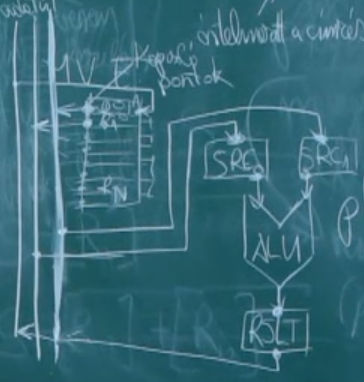
\includegraphics[width=0.8\textwidth]{haromut}
    \centering
    \caption{Háromutas adatút}
    \label{fig:haromut}
\end{figure}

\subsection{Műveletvégző (ALU)}
Az ALU (Aritmetikai Logikai Egység) végzi el a műveleteket.
A leggyakoribb, legelemibb művelet az összeadás.

\subsubsection{Az ALU által végzett műveletek}
\begin{itemize}
    \item FX: + - * /
    \item FP: + - * /
    \item BCD: + - * /
    \item Egyéb: eltolás, negálás, léptetés, logikai műveletek
\end{itemize}

\subsubsection{Összeadó}
Egy félösszeadónak két bemenete és két kimenete van, a második kimenet az átvitelre van (carry).
\begin{figure}[H]
    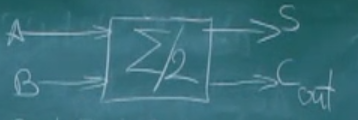
\includegraphics[width=0.8\textwidth]{felossze}
    \centering
    \caption{Félösszeadó}
    \label{fig:felossze}
\end{figure}
A carry bit meghatározásához egy AND kaput használ a félösszeadó (akkor van átvitel, ha mindkét bement 1), az ereményhez pedig egy XOR kaput.
\begin{figure}[H]
    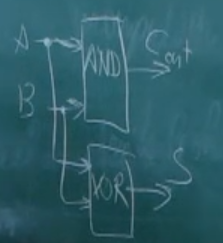
\includegraphics[width=0.8\textwidth]{felosszek}
    \centering
    \caption{Félösszeadó kapujainak felépítése}
    \label{fig:felosszek}
\end{figure}

Teljes összeadónál három bemenet van, hogy az előző összeadás carry kimenetét is figyelembe tudja venni.
\begin{figure}[H]
    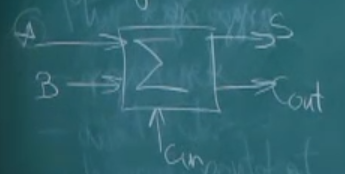
\includegraphics[width=0.8\textwidth]{teljesossze}
    \centering
    \caption{Teljes összeadó}
    \label{fig:teljesossze}
\end{figure}
A teljes összeadó felépíthető félösszeadókból:
\begin{figure}[H]
    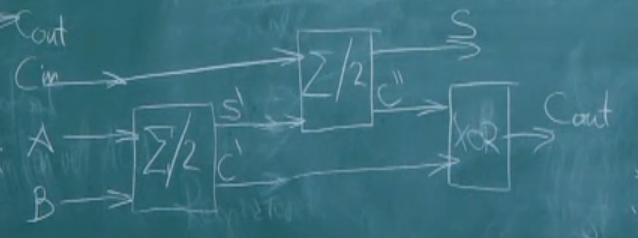
\includegraphics[width=0.8\textwidth]{teljesosszefel}
    \centering
    \caption{Teljes összeadó félösszeadókból}
    \label{fig:teljesosszefel}
\end{figure}
Ez 3 ciklusba kerül, a cél a folyamat gyorsítása.
Az igazságtáblát felírva és a logikai függvényeket egyszerűsítve a következő kapukból építhető fel a teljes összeadó:
\begin{figure}[H]
    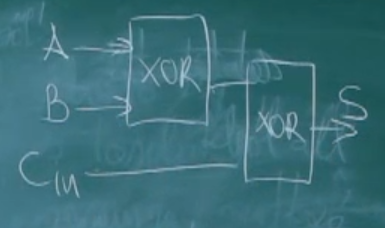
\includegraphics[width=0.8\textwidth]{teljesosszeegyszeru}
    \centering
    \caption{Teljes összeadó egyszerűsítése (eredmény kiszámítása)}
    \label{fig:teljesosszeegyszeru}
\end{figure}
\begin{figure}[H]
    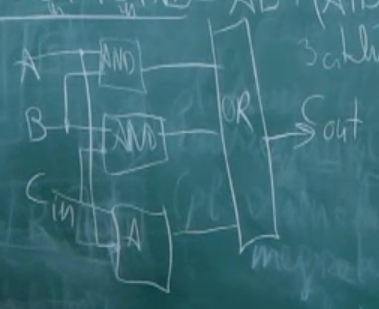
\includegraphics[width=0.8\textwidth]{teljesosszeegyszeruc}
    \centering
    \caption{Teljes összeadó egyszerűsítése (carry kiszámítása)}
    \label{fig:teljesosszeegyszeruc}
\end{figure}
Ezzel a művelet már két óraciklus alatt is elvégezhető, azaz a teljesítmény 33\%-kal növekszik.
